
\subsection{Flexible blokken}\label{felix}
\pvelist{ \pve{2.7} }
Het is voor redacteuren mogelijk om blokken de plaatsen op pagina's. Hiermee krijgt de redacteur enige vrijheid over de indeling van de pagina. Hier zijn wel beperkingen van toepassing volgens het grafisch ontwerp.

Door met de muis over de grijze balk te gaan verschijnt er een tandwieltje, als je daarop klikt dan verschijnt er een optie \emph{Blok toevoegen}. Hier kan een keuze gemaakt worden om een enkel item weer te geven op de website, dit zijn \emph{Nodetypes}, of een aantal items, zoals bijvoorbeeld \emph{Het laatste nieuws}.

\begin{figure}[p]
\centering
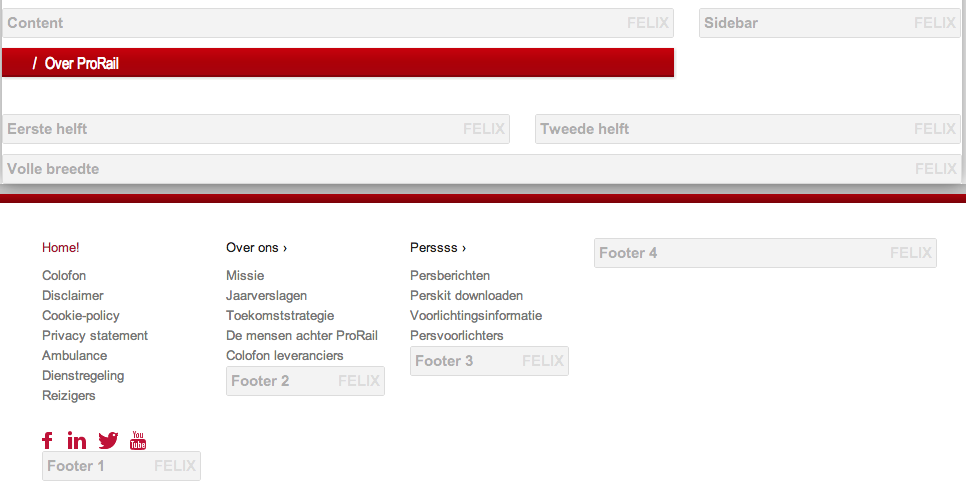
\includegraphics[width=\textwidth]{img/felix.png}
\caption{De grijze balken met het woord FELIX erin zijn de gebieden waar de redacteur blokken kan plaatsen}
\label{fig:felix_image}
\end{figure}

\subsubsection{Woordvoerders}
Er kunnen personen worden uitgelicht via Felix. Kies voor woordvoerders. Er dient nu een keuze gemaakt te worden. Deze lijst kan men samenstellen via \drupalpath{admin/structure/taxonomy/activiteiten\_van\_prorail}. Bij het aanmaken of toevoegen van een persoon kan je een persoon indelen in een van de activiteiten die in die lijst staan.

\subsubsection{Banner}
In de regio banner kan via Felix een Redactioneel blok geplaatst worden. Bij het toevoegen van het blok is het blok zichtbaar op het domein waar je op dat moment bevindt; er wordt een blok toegevoegd op een nieuwsbericht wat gepubliceerd staat op Reizigers, dat wil dus zeggen dat dat blok over het gehele reizigers domein beschikbaar is. Dit blok is automatisch toegevoegd op de 70/30 verdeling van de pagina, op de 60/40 verdeling dient de redacteur dit zelf nog toe te voegen.

\subsubsection{Beeldengalerij}
Er kan een beeldengalerij geplaatst worden op de website door het content type beeldengalerij in te vullen. Nadat dit gedaan is kan er via Felix deze node worden uitgelicht op de website. Dit kan alleen in de content regio.
%todo: Screenshot maken van Felix add block interface bij oplevering 

\subsubsection{Achtergrondkleur aanpassen}
Klik op het tandwieltje bij een blok en kies voor blok instellingen. Vul dan bij block class \emph{schaduw} in.

\subsubsection{YouTube Blok}
Hij laat altijd de 2 laatste video's van het Prorail-kanaal zien. Je hebt echter als eindredacteur de mogelijkheid om hier wat extra invloed op uit te oefenen door een video bijv sticky/vastgeplakt te maken.

Ook kun je op bepaalde pagina's andere video's tonen door het blok een tagfilter mee te geven. Daarvoor moet je de video's wel tags meegeven en als je het videoblok op een pagina zet een tagfilter meegeven. Dat kan door het blok te bewerken via Edit attributes

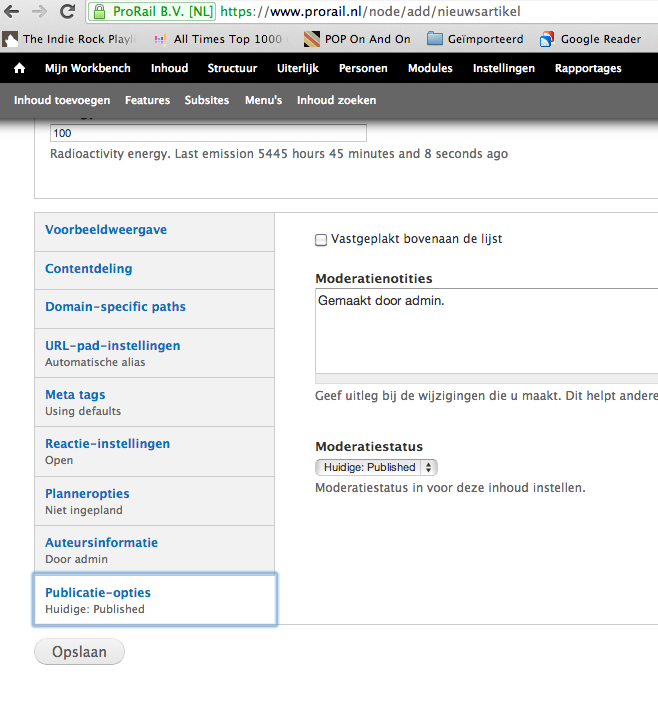
\includegraphics[width=\textwidth]{img/youtubebloksticky.png}
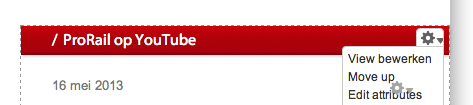
\includegraphics[width=\textwidth]{img/youtubeblok1.png}
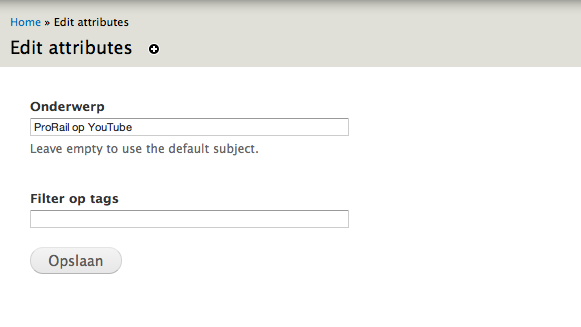
\includegraphics[width=\textwidth]{img/youtubeblok2.png}
